\section{Experiment \& Data Collection} \label{oversky}

The main preliminary steps performed to enable our
work are twofold: 1) domain name collection and 2) per-provider performance
measurement. The
remainder of this section details these steps and the reasoning behind them
while providing context with which to view results presented throughout this paper. 

\begin{figure}
    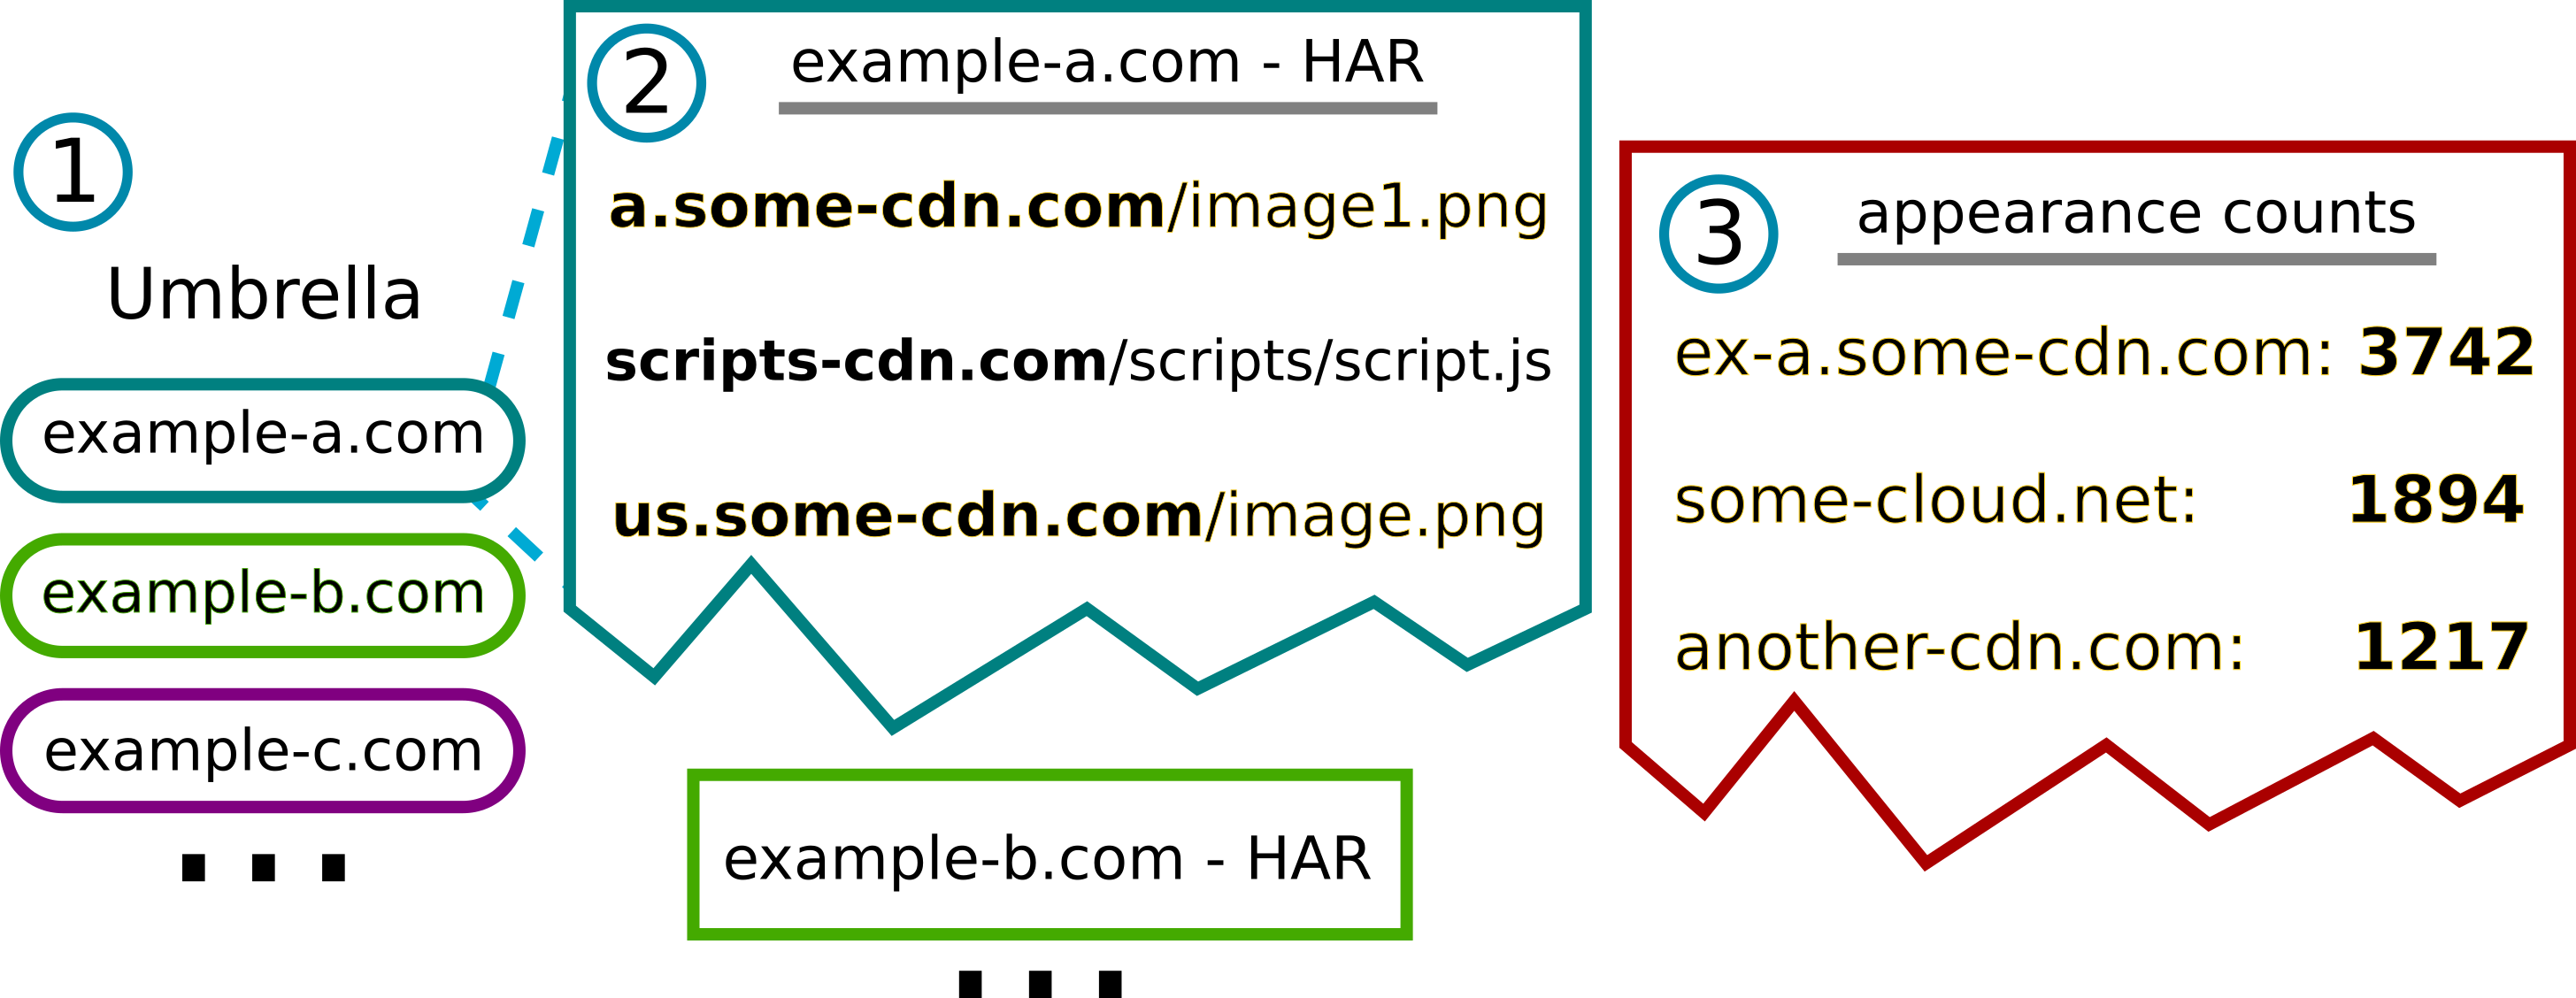
\epsfig{file=figs/domain_finding.png, width=1\linewidth}
    \caption{Diagram illustrating domain name collection: 1) Domains from the Umbrella top 1-million were loaded via Google Chrome to identify human-targeted websites. 2) For each human-targeted website's landing page, a HAR file was recorded. 3) Domains were extracted from HAR data and ranked by the number of times observed.
    }
    \label{fig:domfind}
\end{figure}

\subsection{Definitions}

As our aim in this paper is to explore the cross-provider behavior of Internet
resource-to-client mapping schemes, it is necessary to first establish what
qualifies as ``cross-provider'' and what sort of cross-provider behavior is of
relevance. For example, the reader may have observed that, if a pair of
providers are not used in \emph{together} for a given online experience, there
is no reason not to keep their analyses separate. For the purposes of this
paper, we choose to focus on the providers of webpage objects, which are known
to often span a multitude of providers \cite{butkiewicz2011}. Previous work has well documented
the impact of individual, slow loading objects on page load time \cite{wang2013}. To this
end, we target domains which we empirically found to co-inhabit large numbers of
webpages as web object hosts. Throughout this paper, we equate ``domain'' to
``host'' or ``provider'', recognizing, however, that it is often the case that a
single provider will use several domain aliases. 

Likewise, we also note here that our use of the term ``[web] resource'' is
deliberately ambiguous: the explicit implementation method used by each provider
--- ranging from a single subnet per geographic point-of-presence to a number of
software-partitioned subnets per machine --- is opaque and beyond the scope of
this paper. Our chief concern is that an identifiable distinction is made
between the set of targets (IP addresses) provided in DNS answers: the sheer fact that they are not
labeled as \emph{same} target indicates that there is likely some difference,
performance or otherwise, between them. For simplicity, we treat
each /24 IPv4 subnet (generally, the most fine-grained BGP prefix route
announcement allowed, by convention) as a potentially distinct resource, noting
that it may be the case that larger providers operate with smaller (more coarse
grained) prefixes.

\subsection{Domain Collection}

We use the top 10,000 most frequently resolved domains from Cisco's Umbrella Top
1-Million list \cite{scheitle2018} as a starting point. 
\RF{Would be nice if we can give the date of the list. It is better for reproducibility
, plus some research show that the list may change a lot during weekends }
However, as this list is obtained from
the perspective of DNS resolution, the relationship \emph{between} these domains
is unclear. Further, as there is no complete URL information from such a
perspective, there is no indication which domains are used for downloading web
content, as opposed to providing some other service or interface. To address
this, we attempt to load pages from this list and ultimately use domains
providing web objects discovered on each successfully loaded page. This process
is detailed below and illustrated in Figure \ref{fig:domfind}.

First we attempt to load each web page from the Umbrella list using Google
Chrome. If a page loaded, its source was checked for any indication that the
page was not intended for human use (for example, automated server response
pages for non-200 HTTP status messages). This filter reduced the size of our
domain set from 10,000 pages to 2,441 pages. For each of these pages, a HAR file
(in HTTP Archive format file) was saved to capture the full set of web objects
loaded with the page. By using HAR files instead of just the page source, we
avoid missing any dynamically loaded objects that may not appear in the original
source. 
%Even after using this approach, the space of possible domains remains larger
%than we can address in the scope of this experiment.
The HAR file provides the
full HTTP path of each web object retrieved. Domains used in this experiment
come from this dataset. 

Due to security related rate limits, our experiment was limited to 15-20 domain measurements per
client per day, thus further restricting the number of domains to be used in our
experiment. Since the entire set obtained was large, we \emph{ranked}
object hosting domains by how frequently they were observed across our set of HAR
files. The most frequently appearing object hosting domains were given priority.
Ultimately, 304 domains were used for the work described in this paper. 

\RF{the number 304 still looks very arbitrary?}

\begin{figure}
    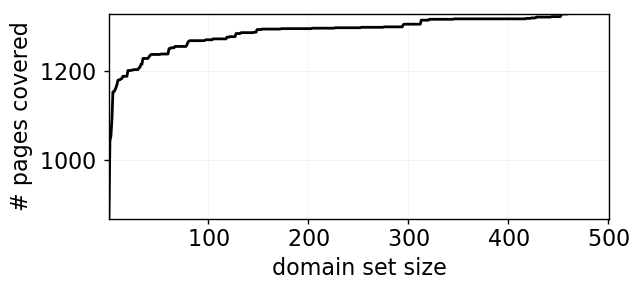
\epsfig{file=figs/num_sites_covered_by_top_n_doms.png, width=1\linewidth}
    \caption{The number of sites containing an object hosted by a domain in our set vs
    the size of our set of domains.}
    \label{fig:sitescovered}
\end{figure}

\begin{figure}
    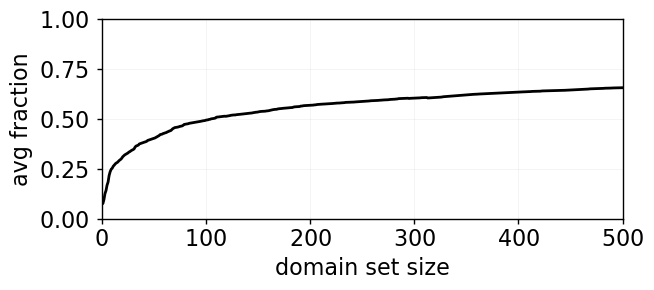
\epsfig{file=figs/fraction_links_covered_by_top_n_doms.png, width=1\linewidth}
    \caption{Mean fraction of page object links (URLs) covered per site vs the
    number of domains used.
    }
    \label{fig:linkscovered}
\end{figure}

In Figues \ref{fig:sitescovered} and \ref{fig:linkscovered}, we show the
decreasing marginal impact of each additional domain in our set. As shown, both
quantities --- the number of visited pages including a URL from our domain set and the
fraction of URLs on each page addressed by our set --- exhibit logarithmic-like
growth patterns, beginning to plateau well before 100 domains are reached. We
assert that this demonstrates the aggregate behavior of the 304 domains obtained above
should sufficiently cover the domain diversity of a ``typical'' popular web page. 


\subsection{Per-Provider Performance Measurement}

Any attempt to identify the general groups that Internet clients are mapped to
requires a dataset with a uniquely broad scope: not only breadth --- a diverse
set of clients --- but also depth --- many clients from each, yet to be
uncovered, group or cluster. In addition, we are required to minimize the
temporal spread of the measurements, as network resource allocation is known to
change over time. We utilize the RIPE Atlas platform \cite{ripe-atlas} for our measurements.
RIPE Atlas offers a large number of globally distributed clients, capable of
performing lightweight network measurements, such as pings, on behalf of
configurable requests received by the Atlas API. We deployed ping measurements
to the previously described 304 domains from 10,274 of RIPE's clients. Each
client performed DNS resolution for pings via their local DNS resolver, ensuring
that they each targeted the web resource they would ordinarily be directed to.

Unavoidable flux in the availability of individual, voluntarily maintained
clients lead to some clients performing only a subset of the given
measurements, thus missing some of the domains of interest. To be sure that this
does not dramatically affect our findings, we arbitrarily enforce minimal amount
of domain coverage --- 160 domains, just more than half of our set --- for use
of a given client's data. We show in Section \ref{sect:cnre} the effects of domain quantity
in our measurements.
